\section{Market Design for a Self-Incentivizing Network}
\label{sec:designs}
we first set out to create the simplest market possible and evaluate its problems to see where to improve.

Desired properties

\begin{itemize}

\item Let anybody contribute capacity

\item Allow users with different utility functions to interact (flow completion time vs.~jitter)

\item Allow users to buy guarantees (and not get swindled)

\end{itemize}

\subsection{Simple Market Design}
we did x. (TODO: include basic inkscape thing)

\subsection{Simple Market Evaluation}

Simulation experiments to test whether the one-layer market has each desired property?

Measure outcome quality (vs.~SRTF or other optimal), \# of roundtrips

can simulate multiple users with different objectives

\begin{figure}
%\vspace{\baselineskip}
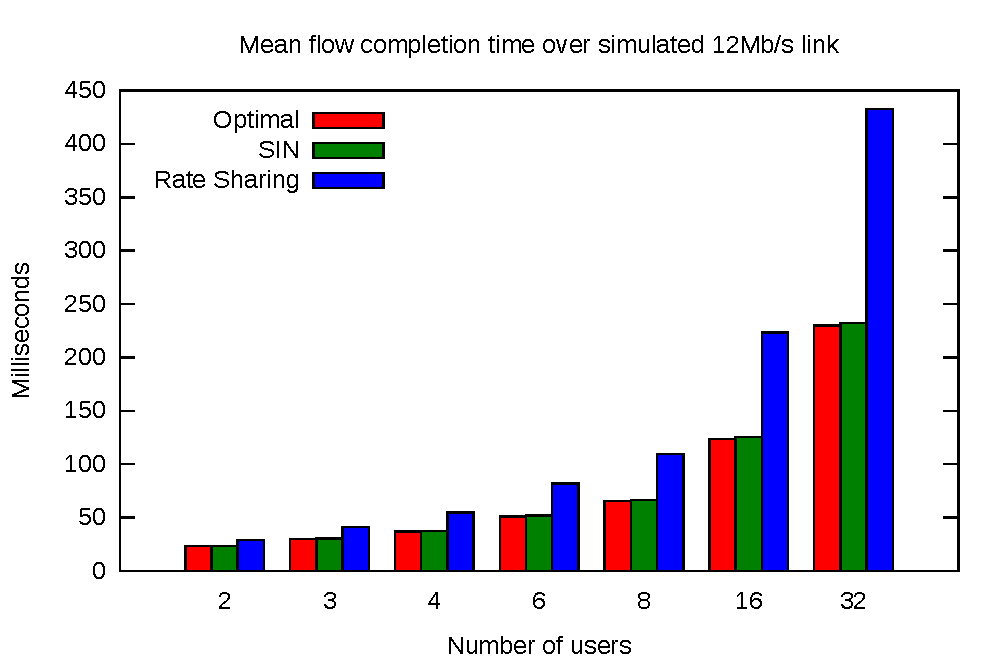
\includegraphics[width=\columnwidth]{plots/delay_over_srtf.pdf}
\caption{Average queuing delay of simlulations divided by the average queuing delay of the optimal shortest remaining time first solution.}
\label{f:delay_over_srtf}
\end{figure}

\begin{figure}
%\vspace{\baselineskip}
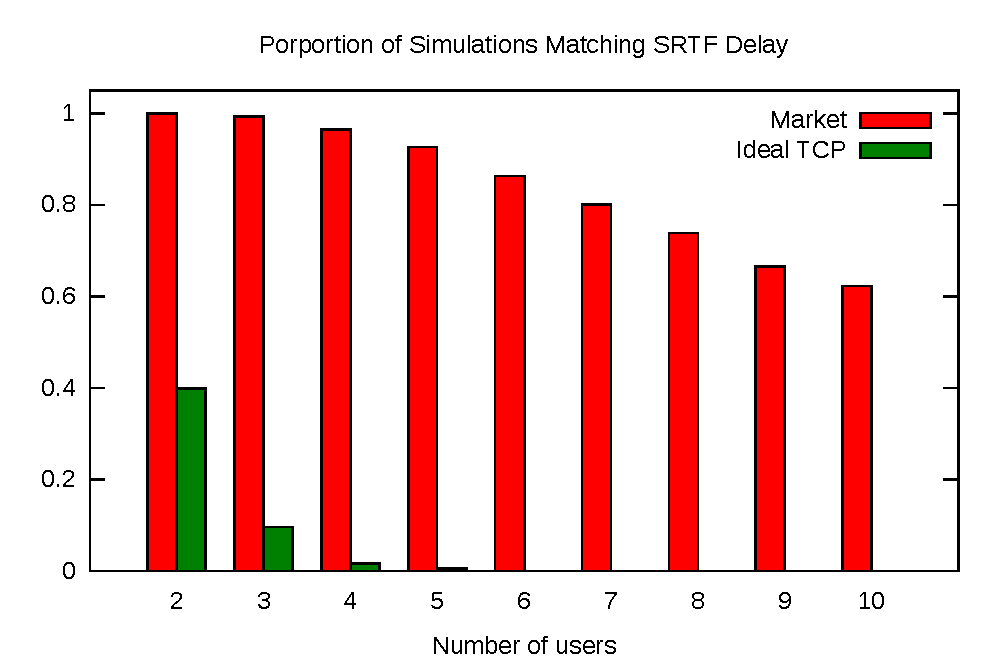
\includegraphics[width=\columnwidth]{plots/percent_match_srtf.pdf}
\caption{Percent of simlulations that achieved optimal shortest remaining time first solution.}
\label{f:percent_match_srtf}
\end{figure}

We simulated the results of running a market in practice with users that would arrive at time $t$ had a known number of packets $n$ they wanted to send.
Their utility is defined as:.
Figures~\ref{f:delay_over_srtf} and \ref{f:percent_match_srtf} show the result of running the simulation with 2 to 10 concurrent users, all trying to minimize their flow completion time for the cheapest cost.
We compare with a round robin scheme, which is the ideal equillibrium of mutliple TCP flows and a FIFO queued router (TODO cite).
In our simulations, there are a varying number of users with a flow start time chosen from a uniform random distribution between 0 and 9 with flow lengths chosen from a uniform random distribution between 1 and 10. We compare to the allocation of packets to times that minimizes the queued time for each flow: shortest remaining time first scheduling (TODO cite).

We find that bots in our market almost always converge on an allocation that is equivalent to the optimal shortest remaining time first schedule when there is a small number of users. Larger numbers of users are less likely to achieve an optimal solution, but the excess queuing delay over the optimal SRTF solution remains extremely low with a large number of users: less than 1\% overhead in all of our evaluations.

problem with current design, introduce evil user
problem: exposure problem, evil user

the problems we encountered with the simple market led us to our current design:
\subsection{Multi-Layer Market Design}

Sketch of multi-layer design
